% CS70--Spring 2024 --- Discussion 2A Solutions
\documentclass[11pt]{article}
\usepackage{amsmath,textcomp,amssymb,geometry,graphicx,enumerate}
\usepackage{xeCJK}

\def\Name{JayZhao}  % Your name
\def\SID{0}  % Your student ID number-
\def\Homework{2A} % Number of Homework
\def\Session{Spring 2024}

\title{CS70--Spring 2024 --- Discussion \Homework \ Solutions}
\author{\Name, SID \SID}
\markboth{CS70--\Session\  Discussion \Homework\ \Name}{CS70--\Session\ Discussion \Homework\ \Name}
\pagestyle{myheadings}
\date{\today}

\newenvironment{qparts}{\begin{enumerate}[{(}a{)}]}{\end{enumerate}}
\def\endproofmark{$\Box$}
\newenvironment{proof}{\par{\bf 证明}:}{\endproofmark\smallskip}

\textheight=9in
\textwidth=6.5in
\topmargin=-.75in
\oddsidemargin=0.25in
\evensidemargin=0.25in

\begin{document}
\maketitle


% 1. 欧拉回路与欧拉路径
\section*{1. 欧拉回路与欧拉路径}
\begin{figure}
    \centering
    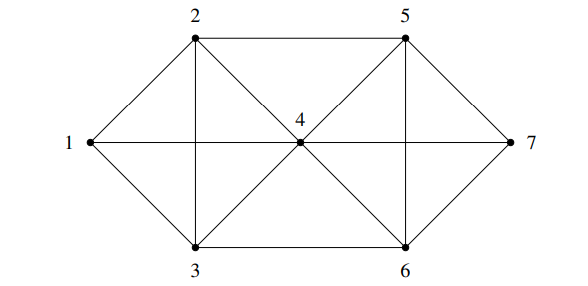
\includegraphics[width=0.5\linewidth]{week2/image.png}
\end{figure}
\begin{qparts}
\item 上图中是否存在欧拉回路?如果不存在,请给出理由。如果存在,请提供一个例子。

\begin{proof}
欧拉回路是指一条经过图中每条边恰好一次并回到起点的回路。对于无向图,存在欧拉回路的充要条件是:图是连通的,且所有顶点的度均为偶数。\newline
观察图中各顶点的度,若存在至少一个顶点的度为奇数,则不存在欧拉回路。\newline
点1和点7的度为奇数,因此,本图不存在欧拉回路,因为存在度为奇数的顶点。
\end{proof}

\item 上图中是否存在欧拉路径?如果不存在,请给出理由。如果存在,请提供一个例子。

\begin{proof}
欧拉路径是指一条经过图中每条边恰好一次的路径(不要求回到起点)。对于无向图,存在欧拉路径的充要条件是:图是连通的,且恰有0个或2个奇数度顶点。\newline
若图中恰有2个奇数度顶点,则存在欧拉路径,且该路径的起点和终点分别为这两个奇数度顶点。\newline
因此,本图存在欧拉路径。例如:142312543647567
\end{proof}

\item 无向图中存在欧拉路径的条件是什么?请简要证明你的答案。

\begin{proof}
设$G$为一个连通的无向图。我们证明:$G$存在欧拉路径当且仅当$G$中恰有0个或2个奇数度顶点。

\textbf{必要性}:
假设$G$存在一条欧拉路径$P$,该路径从顶点$s$出发,到顶点$t$结束($s$可以等于$t$)。
在$P$中,除了$s$和$t$以外的每个顶点,进入和离开该顶点的次数都相等,因此这些顶点的度为偶数。
若$s \neq t$,则$s$和$t$各有一条边只被经过一次(分别为起点和终点),因此它们的度为奇数。
若$s = t$,则所有顶点的度都为偶数。
因此,$G$中奇数度顶点的个数只能为0或2。

\textbf{充分性}:
若$G$中没有奇数度顶点,则所有顶点度为偶数。根据欧拉定理,$G$存在欧拉回路,欧拉回路也是欧拉路径的一种特殊情形。
若$G$中恰有2个奇数度顶点,设为$s$和$t$。我们可以在$G$中添加一条边$e$,连接$s$和$t$,得到新图$G'$。此时$G'$所有顶点度均为偶数,且$G'$仍然连通,因此$G'$存在欧拉回路。
在$G'$的欧拉回路中,去掉添加的边$e$,就得到$G$中一条从$s$到$t$的欧拉路径。

综上,$G$存在欧拉路径当且仅当$G$连通且奇数度顶点数为0或2。
\end{proof}

\end{qparts}

% 2. 树的着色
\section*{2. 树的着色}

\begin{qparts}
\item 证明所有至少有2个顶点的树都至少有两个叶节点。

\begin{proof}
设$T$为一棵至少有2个顶点的树。\newline
任选$T$中一条最长路径$P$,设其两个端点为$u$和$v$。若$u$的度大于1,则存在一条从$u$出发且不在$P$上的边,连接到某顶点$w$,则$w$不在$P$上,将$w$加入$P$可得到更长路径,矛盾。因此$u$的度为1,同理$v$的度也为1。\newline
所以$T$至少有两个叶节点。
\end{proof}

\item 证明所有至少有2个顶点的树都是二分图。

\begin{proof}
用数学归纳法证明。\newline
\textbf{基础情形}:当树有2个顶点时,只有一条边,显然是二分图。\newline
\textbf{归纳假设}:假设任意$n$个顶点的树是二分图。\newline
\textbf{归纳步骤}:考虑$n+1$个顶点的树$T$。$T$必有一个叶节点$v$,去掉$v$及其唯一相邻顶点$u$之间的边,得到$n$个顶点的树$T'$。由归纳假设,$T'$是二分图,设其二分为$A,B$。将$v$加入到与$u$不同的集合即可,$T$仍为二分图。\newline
因此,所有树都是二分图。
\end{proof}
\end{qparts}

% 3. 度序列
\section*{3. 度序列}

在判断一个度序列是否可以对应某个简单无向图时,常用的方法之一是\textbf{Havel-Hakimi算法}。该算法的基本思想如下:

\begin{itemize}
  \item 首先将度序列按降序排列。
  \item 取出序列中最大的度$d$,并将其从序列中删除。
  \item 将剩下的前$d$个数各减1(表示与最大度顶点相连)。
  \item 若此过程中出现负数或无法继续,则该度序列不可实现;若最终所有度数都为0,则该度序列可实现。
\end{itemize}

图的度序列是其所有顶点的度的序列,按降序排列,并根据需要包含重复项。例如,以下图的度序列是 (3,2,2,2,1)。
\begin{center}
  \includegraphics[width=0.25\linewidth]{week2/image2.png}
\end{center}
对于下面的每个部分,判断是否存在一个具有给定度序列的简单无向图$G$(即没有自环和重边)。请证明你的论断。

\begin{qparts}
\item $(3,3,2,2)$

\begin{proof}
首先,度数之和为$3+3+2+2=10$,是偶数,满足无向图的必要条件。\newline
使用Havel-Hakimi算法:取最大度3,去掉它并将其与其他3个顶点相连,剩下度数为$(2,1,1)$。再取2,去掉它并与剩下两个顶点相连,剩下$(0,0)$。所有度数均为0,算法结束。\newline
因此,存在这样的简单无向图。例如,顶点$A,B$度为3,$C,D$度为2,边为$AB,AC,AD,BC,BD,CD$。
\end{proof}

\item $(3,2,2,2,2,1,1)$

\begin{proof}
度数之和为$3+2+2+2+2+1+1=13$,是奇数。\newline
无向图的度数和必须为偶数(每条边贡献2),因此不存在这样的简单无向图。
\end{proof}

\item $(6,2,2,2)$

\begin{proof}
度数之和为$6+2+2+2=12$,是偶数。\newline
但顶点数为4,最大度不能超过$4-1=3$,而6大于3,矛盾。\newline
因此,不存在这样的简单无向图。
\end{proof}

\item $(4,4,3,2,1)$

\begin{proof}
度数之和为$4+4+3+2+1=14$,是偶数。\newline
使用Havel-Hakimi算法:取4,去掉它并与剩下4个顶点相连,剩下$(3,2,1,0)$。再取3,去掉它并与剩下3个顶点相连,剩下$(1,0,0)$。再取1,去掉它并与剩下一个顶点相连,剩下$(0,0)$。但在实际构造时,最后一个度为1的顶点只能与度为0的顶点相连,矛盾。\newline
因此,不存在这样的简单无向图。
\end{proof}
\end{qparts}
\end{document} 